\section{Conflicts}
\subsection{Shift-Reduce conflict}
Given an m-state, there is a S-R conflict if there is an arc with label $a$, as well as a final state with $a$ in the lookahead set.
\begin{figure}[H]
    \centering
    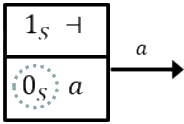
\includegraphics[width=0.2\linewidth]{parsing/shift-reduce-conflict.png}
\end{figure}

\subsection{Reduce-Reduce conflict}
Given an m-state, there are 2 final candidates with a non-empty intersection of the lookahead sets.
\begin{figure}[H]
    \centering
    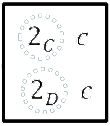
\includegraphics[width=0.15\linewidth]{parsing/reduce-reduce-conflict.png}
\end{figure}

\subsection{Convergent arcs with conflict}
Given 2 candidates in the same m-state, with non-empty intersection lookaheads, which go with a convergent arc to the same final m-state.
\begin{figure}[H]
    \centering
    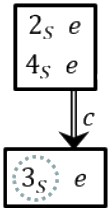
\includegraphics[width=0.15\linewidth]{parsing/convergent-conflict.png}
\end{figure}
